Vi skal se på tre typer filtre: Butterworth, Bessel og Chebyshev.
De forskjellige typene har forksjellige egenskaper som velges etter
hvilke egenskaper som passer formålet.

\begin{figure}[H]
  \caption{Filtertyper}
  \centering
  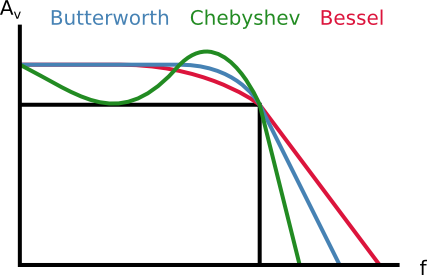
\includegraphics[width=0.67\textwidth]{./img/filtertyper}
\end{figure}

\paragraph{Butterorth (Maximally flat)} \mbox{} \\
+ Flat respons $A_v$ relativt konstant innenfor båndet). \\
+ Mest brukte aktive filteret. \\
- Fasegang endres når filteret avtar.

\paragraph{Bessel} \mbox{} \\
+ Konstant fasegang. \\
+ HiFi (High Fidelity).

\paragraph{Chebyshev} \mbox{} \\
+ Bratt rolloff. \\
- Ikke konstant spenningsforsterkning.
